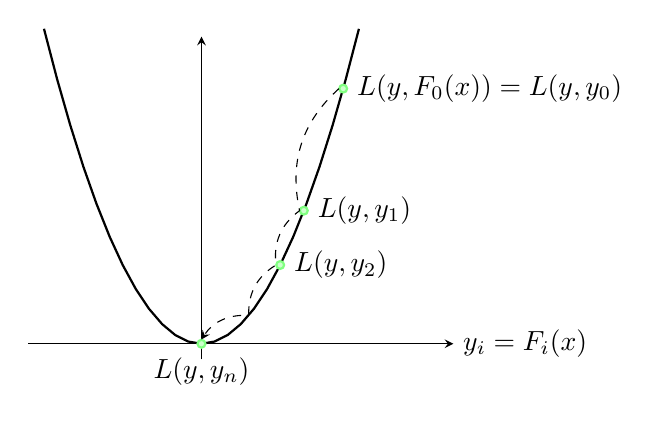
\begin{tikzpicture}
    [place/.style={circle,scale=0.3,draw=green!50,fill=green!20,thick},
    transition/.style={rectangle,draw=black!50,fill=black!20,thick}]

    %\draw[help lines] (-2.9,-0.2) grid (2.9,3.9);
    \draw[->,>=stealth] (-2.2,0) -- (3.2,0) node[right] {$y_i=F_i(x)$};
    \draw[->,>=stealth] (0,-0.2) -- (0,3.9);
    \draw[thick,color=black,domain=-2:2] plot (\x,\x*\x);

    \node[place,label=right:{$L(y,F_0(x)) = L(y, y_0)$}] (f0) at (1.8,3.24)  {};
    \node[place,label=right:{$L(y,y_1)$}] (f1) at (1.3,1.69)  {};
    \node[place,label=right:{$L(y,y_2)$}] (f2) at (1.0,1.0)   {};
    \node[place,label=below:{$L(y,y_n)$}] (fn) at (0,0)  {};

    \draw[->,>=stealth,dashed] (f0.west) to[bend right] (f1.west)
          to[bend right] (f2.west)
          to[bend right] (0.6,0.36)
          to[bend right] (fn.north);
\end{tikzpicture}
